\documentclass[dvisvgm]{standalone}
\usepackage{tikz}
\usepackage{pgfplots}

\begin{document}
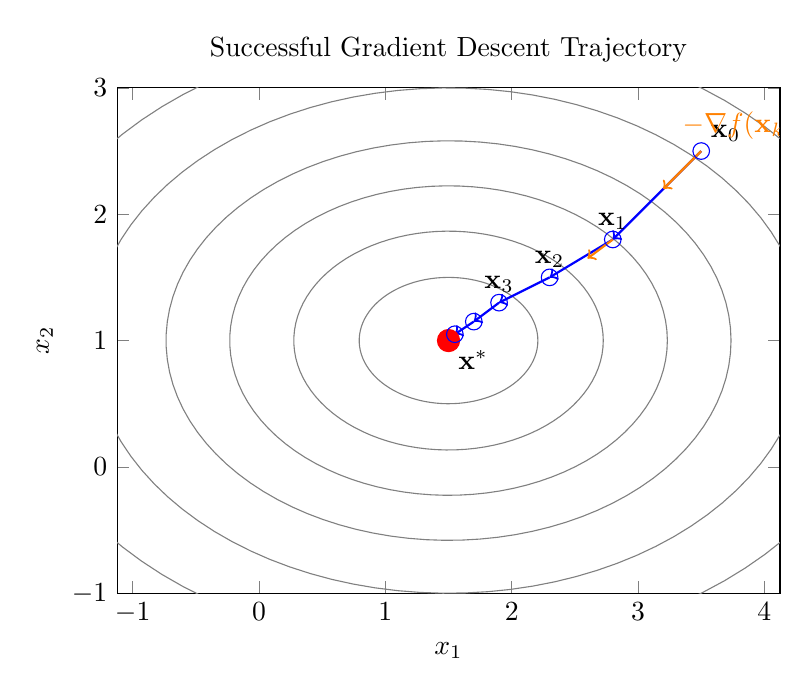
\begin{tikzpicture}
    \begin{axis}[
        width=10cm,
        height=8cm,
        xlabel={$x_1$},
        ylabel={$x_2$},
        grid=none,
        axis equal,
        xmin=-1, xmax=4,
        ymin=-1, ymax=3,
        title={Successful Gradient Descent Trajectory}
    ]
    
    % Draw contour lines (elliptical, well-conditioned)
    \foreach \level in {0.5, 1.5, 3, 5, 8, 12, 17, 23}
    {
        \addplot[gray, thin, domain=0:360, samples=100] 
            ({1.5 + sqrt(\level)*cos(x)}, {1 + sqrt(\level/2)*sin(x)});
    }
    
    % Mark the minimum
    \addplot[red, mark=*, mark size=4pt, only marks] coordinates {(1.5, 1)};
    \node at (axis cs:1.5,1) [below right] {$\mathbf{x}^*$};
    
    % Optimization trajectory points
    \coordinate (x0) at (axis cs:3.5, 2.5);
    \coordinate (x1) at (axis cs:2.8, 1.8);
    \coordinate (x2) at (axis cs:2.3, 1.5);
    \coordinate (x3) at (axis cs:1.9, 1.3);
    \coordinate (x4) at (axis cs:1.7, 1.15);
    \coordinate (x5) at (axis cs:1.55, 1.05);
    \coordinate (x6) at (axis cs:1.5, 1);
    
    % Draw trajectory
    \draw[->, thick, blue] (x0) -- (x1);
    \draw[->, thick, blue] (x1) -- (x2);
    \draw[->, thick, blue] (x2) -- (x3);
    \draw[->, thick, blue] (x3) -- (x4);
    \draw[->, thick, blue] (x4) -- (x5);
    \draw[->, thick, blue] (x5) -- (x6);
    
    % Mark iteration points
    \addplot[blue, mark=o, mark size=3pt, only marks] coordinates 
        {(3.5, 2.5) (2.8, 1.8) (2.3, 1.5) (1.9, 1.3) (1.7, 1.15) (1.55, 1.05)};
    
    % Add labels
    \node at (axis cs:3.5, 2.5) [above right] {$\mathbf{x}_0$};
    \node at (axis cs:2.8, 1.8) [above] {$\mathbf{x}_1$};
    \node at (axis cs:2.3, 1.5) [above] {$\mathbf{x}_2$};
    \node at (axis cs:1.9, 1.3) [above] {$\mathbf{x}_3$};
    
    % Add gradient vectors at a few points
    \draw[->, thick, orange] (axis cs:3.5, 2.5) -- (axis cs:3.2, 2.2);
    \draw[->, thick, orange] (axis cs:2.8, 1.8) -- (axis cs:2.6, 1.65);
    \node at (axis cs:3.8, 2.7) [orange] {$-\nabla f(\mathbf{x}_k)$};
    
    \end{axis}
\end{tikzpicture}
\end{document}
